% Created 2017-10-21 Sat 09:26
% Intended LaTeX compiler: pdflatex
\documentclass[11pt]{article}
\usepackage[utf8]{inputenc}
\usepackage[T1]{fontenc}
\usepackage{graphicx}
\usepackage{grffile}
\usepackage{longtable}
\usepackage{wrapfig}
\usepackage{rotating}
\usepackage[normalem]{ulem}
\usepackage{amsmath}
\usepackage{textcomp}
\usepackage{amssymb}
\usepackage{capt-of}
\usepackage{hyperref}
\usepackage{minted}
\author{Raynold Ng}
\date{2017/10/14}
\title{Introduction to TensorFlow\\\medskip
\large Hackerschool, NUS Hackers}
\hypersetup{
 pdfauthor={Raynold Ng},
 pdftitle={Introduction to TensorFlow},
 pdfkeywords={},
 pdfsubject={},
 pdfcreator={Emacs 25.2.1 (Org mode 9.0.9)}, 
 pdflang={English}}
\begin{document}

\maketitle
\section*{Agenda}
\label{sec:orgc63bbd7}
\begin{itemize}
\item Installation and Setup
\item Machine Learning Primer
\item What's TensorFlow?
\item Basic TensorFlow concepts
\item MNIST Example
\begin{itemize}
\item Softmax
\item Convoluted Neural Networks
\end{itemize}
\end{itemize}
\section*{Installation and Setup}
\label{sec:orgdc4fc67}

Ensure that you have the following installed:
\begin{enumerate}
\item TensorFlow: \url{https://www.tensorflow.org/install/}
\item Python 3: \url{https://www.python.org/downloads/}
\item Jupyter (recommended): \url{http://jupyter.org/}
\end{enumerate}

Materials are available \href{https://github.com/raynoldng/hackerschool-tensorflow}{here}
\section*{Machine Learning Primer}
\label{sec:org6b8b5f4}
\subsection*{What is Machine Learning?}
\label{sec:orgd9b94fb}
\begin{itemize}
\item "The science of getting computers to act \textbf{without being explicitly programmed}" - Andrew Ng
\item Primary aim is to allow computers to learn automatically without human
intervention or assistance and adjust actions accordingly
\end{itemize}
\subsection*{Using TensorFlow to sort cucumbers}
\label{sec:org7463012}
\begin{itemize}
\item \href{https://cloud.google.com/blog/big-data/2016/08/how-a-japanese-cucumber-farmer-is-using-deep-learning-and-tensorflow}{Makoto Koike} used deeping learning and TensorFlow to sort cucumbers by size, shape, color and other attributes
\end{itemize}

\begin{center}
\begin{center}
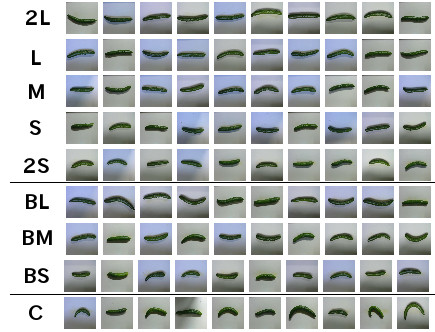
\includegraphics[width=.9\linewidth]{images/cucumber.png}
\end{center}
\end{center}

\subsection*{Structure in data}
\label{sec:org5a8c725}
\begin{itemize}
\item some interpretations to "structure in data"
\begin{itemize}
\item given some data, one can predict other data points with some confidence
\item one can compress the data, i.e., store the same amount of information, with
less space
\end{itemize}
\end{itemize}

\begin{align*}
A = \{1, 2, 6, 4, 7, 9, 0\} \\
B = \{1, 2, 1, 2, 1, 2, 1\}
\end{align*}

\begin{itemize}
\item we might say that \(A\) has apparent structure while \(B\) does not
\end{itemize}

\subsubsection*{Entropy}
\label{sec:org5e1befa}
\begin{itemize}
\item quantified as Entropy of Process
\end{itemize}
$$H(X) = -\sum_{i=1}^{N} p(x_i) \log p(x_i)$$
\begin{itemize}
\item If entropy increases, uncertainty in prediction increases
\end{itemize}
\subsubsection*{Entropy (examples)}
\label{sec:orgcf12476}
\begin{itemize}
\item Example: fair dice
\end{itemize}
$$H(\text{fair dice roll}) = -\sum_{i=1}^6 \frac{1}{6} \log \frac{1}{6}=2.58$$
\begin{itemize}
\item Example: biased 20:80 coin
\end{itemize}
$$H(20/80 \text{ coin toss}) = -\frac{1}{5}\log \frac{1}{5}-\frac{4}{5}\log \frac{4}{5} = 0.72$$
\begin{itemize}
\item biased coin toss has lower entropy; predicting its outcome is easier than a fair dice
\end{itemize}
\subsection*{What are Tensors?}
\label{sec:org1a7df10}
Recall from linear algebra that:
\begin{itemize}
\item Scalar: an array in 0-D
\item Vector: an array in 1-D
\item Matrix: an array in 2-D
\end{itemize}

All are \textbf{tensors} of n-order. Similary, tensors can be transformed with
operations. TensorFlow provides library of algorithms to perform tensor operations efficiently. 
\subsection*{Example}
\label{sec:org1812353}
Simple linear regression model:

$$w_o + w_1 x = \hat{y}$$

\begin{itemize}
\item \(w_0\) and \(w_1\) are \textbf{weights}, that are determined during training
\item \(\hat{y}\) is the predicted outcome, to be compared with actual observations \(y\)
\item Goal: build a model that can find values of \(w_0\) and \(w_1\) that minimize prediction error
\end{itemize}
\subsection*{Graph Representation of ML Models}
\label{sec:orgc986e7a}

Can represent linear regression as a graph

\begin{center}
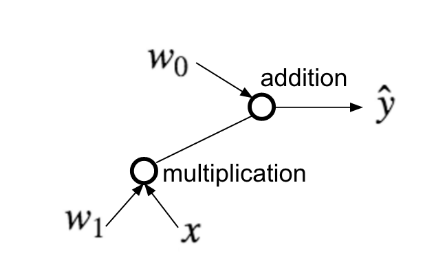
\includegraphics[width=.9\linewidth]{images/linear_reg_graph.png}
\end{center}

\begin{itemize}
\item operations are represented as nodes
\item graph shows how data is transformed by nodes and what is passed between them
\end{itemize}
\subsection*{Graph Representation of ML Models (1)}
\label{sec:orgc184643}
Consider a slightly larger neural net graph:
\begin{center}
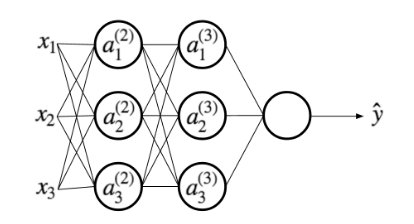
\includegraphics[width=.9\linewidth]{images/neural_net.png}
\end{center}

For more complex models, it could be helpful to visualize your graph.
\href{https://www.tensorflow.org/versions/r0.7/how\_tos/graph\_viz/index.html}{TensorBoard} provides this virtualization tool
\subsection*{Activation Functions}
\label{sec:org2106bdf}
\begin{itemize}
\item A popular function is the rectified linear unit (\textbf{ReLU}):
\end{itemize}
$$g(u) = max(0, u)$$

\begin{center}
\begin{center}
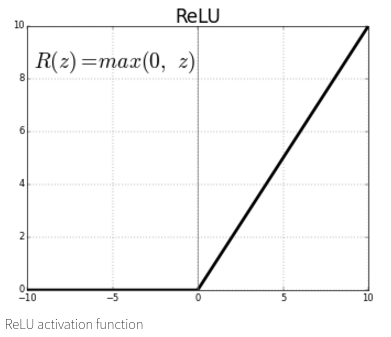
\includegraphics[width=.9\linewidth]{images/relu.png}
\end{center}
\end{center}

\subsection*{Model Output}
\label{sec:org67ea5da}
\begin{itemize}
\item output depends on activation function used, but is generally any real number \([-\infty, \infty]\)
\item For binary classification, an additional sigmoid function can be applied to
bring the output to range of \([0,1]\)
\end{itemize}
$$S(x) = \frac{1}{1+e^{-x}}$$

\begin{center}
\begin{center}
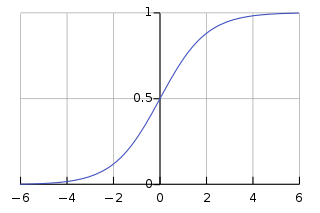
\includegraphics[width=.9\linewidth]{images/sigmoid.png}
\end{center}
\end{center}
\subsection*{Softmax Function}
\label{sec:org538a7a5}
\begin{itemize}
\item for multi-class prediction a softmax function is used:
\end{itemize}
$$S_j(\boldsymbol{z}) = \frac{e^{z_j}}{\sum_{k=1}^K e^{z_k}} \text{ for }j=1,\dots,k$$
\begin{itemize}
\item squash \(K\) dimensional vector \textbf{z} to a \(K\) dimensional vector that sum to 1
\end{itemize}
$$\sum_{j=1}^k S_j(\boldsymbol{z}) = 1$$
\begin{itemize}
\item state usually represented with \textbf{one-hot encoding}, e.g for dice roll \((0,0,1,0,0,0)\)
\end{itemize}
\section*{Basic TensorFlow Concepts}
\label{sec:orgcfc25cb}
\subsection*{What is TensorFlow?}
\label{sec:org6fec455}
\begin{itemize}
\item It is Google's AI Engine
\item "TensorFlow is an interface for expressing machine learning algorithms, and an implementation for executing such algorithms"
\item Originally developed Google Brain Team to conduct machine learning research and deep neural networks research
\item General enough to be applicable to a wide variety of other domains
\end{itemize}
\subsection*{Data Flow Graphs}
\label{sec:orgb9d4191}
Tensorflow separates definition of computations from their execution

Phases:
\begin{enumerate}
\item assemble the graph
\item use a \texttt{session} to execute operations in the graph
\end{enumerate}

\begin{minted}[]{python}
import tensorflow as tf
a = tf.add(3,5)
\end{minted}

\subsection*{How to get value of \texttt{a}?}
\label{sec:org2014023}
\begin{minted}[]{python}
print(a)
\end{minted}

Create a \texttt{session}, and within it, evaluate the graph

\begin{minted}[]{python}
sess = tf.Session()
print(sess.run(a))
sess.close()
\end{minted}

Alternatively:

\begin{minted}[]{python}
with tf.Session() as sess:
    print(sess.run(a))
\end{minted}

\subsection*{Visualizing with TensorBoard}
\label{sec:org137f65c}

\begin{itemize}
\item \texttt{tf.summary.FileWriter} serializes the graph into a format the TensorBoard can read
\end{itemize}

\begin{minted}[]{python}
tf.summary.FileWriter("logs", tf.get_default_graph()).close()
\end{minted}

\begin{itemize}
\item in the same directory, run:
\end{itemize}

\begin{minted}[]{sh}
tensorboard --logdir=logs
\end{minted}

\begin{itemize}
\item This will launch an instance of TensorBoard that you can access at \url{http://localhost:6006}
\end{itemize}

\subsection*{Practice with More Graphs}
\label{sec:orgc6faade}

Try to generate the following graph: (insert equation)

\begin{center}
\begin{center}
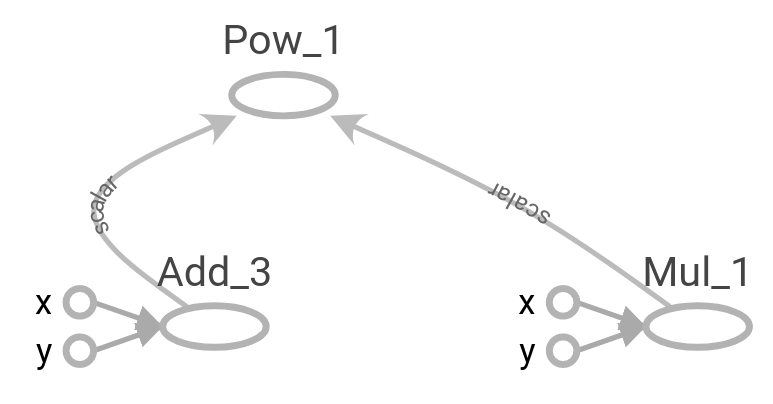
\includegraphics[width=.9\linewidth]{images/graph2.png}
\end{center}
\end{center}

Useful functions: \texttt{tf.add}, \texttt{tf.multiply}, \texttt{tf.pow}

\subsection*{Solution}
\label{sec:org55c325d}

\begin{minted}[]{python}
x = 2
y = 3
op1 = tf.add(x, y)
op2 = tf.multiply(x, y)
op3 = tf.pow(op1, op2)
with tf.Session() as sess:
    op3 = sess.run(op3)
\end{minted}

\subsection*{TensorFlow Variables}
\label{sec:orge4f5913}

\begin{itemize}
\item TensorFlow variables used to represent shared, persistant state manipulated by your program
\item variables hold and update parameters in your model during training
\item variables contain tensors
\end{itemize}

\begin{minted}[]{python}
W1 = tf.ones((2,2))
W2 = tf.Variable(tf.zeros((2,2)), name="weights")

with tf.Session() as sess:
    print(sess.run(W1))
    sess.run(tf.global_variables_initializer())
    print(sess.run(W2))
\end{minted}

\subsection*{Updating Variable State}
\label{sec:org4fbe671}

Use \texttt{tf.assign} to assign a value to a variable

\begin{minted}[]{python}
state = tf.Variable(0, name="counter")
new_value = tf.add(state, tf.constant(1))
update = tf.assign(state, new_value)

with tf.Session() as sess:
    sess.run(tf.global_variables_initializer())
    print(sess.run(state))
    for _ in range(3):
        sess.run(update)
        print(sess.run(state))
\end{minted}

\subsection*{Fetching Variable State}
\label{sec:org25332dc}

\begin{minted}[]{python}
input1 = tf.constant(3.0)
input2 = tf.constant(2.0)
input3 = tf.constant(5.0)
intermed = tf.add(input2, input3)
mul = tf.multiply(input1, intermed)

with tf.Session() as sess:
    result = sess.run([mul, intermed])
    print(result)
\end{minted}

\subsection*{TensorFlow Placeholders}
\label{sec:org4ff502b}

\begin{itemize}
\item \texttt{tf.placeholder} variables represent our input data
\item \texttt{feed\_dict} is a python dictionary that maps \texttt{tf.placeholder} variables to data
\end{itemize}

\begin{minted}[]{python}
input1 = tf.placeholder(tf.float32)
input2 = tf.placeholder(tf.float32)

output = tf.multiply(input1, input2)

with tf.Session() as sess:
    print(sess.run([output], feed_dict={input1:[7.], input2:[2.]}))
\end{minted}

\subsection*{Example: Linear Regression}
\label{sec:orgb030c72}
\subsubsection*{Recap}
\label{sec:orged185f8}
\begin{itemize}
\item we have two weights \(w_0\) and \(w_1\), we want the model to figure out good weights by minimizing prediction error
\item define the following \textbf{loss function}
\end{itemize}

$$L = \sum (y - \hat{y})^2$$

Supose we want to model the following "unknown" function:

$$y = x + 20 \sin(x/10)$$
\subsubsection*{Scatter Plot}
\label{sec:org140efc6}
\begin{center}
\begin{center}
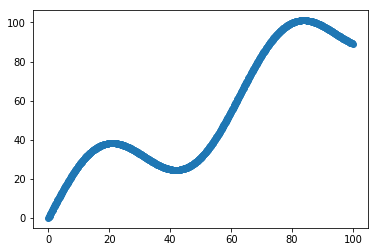
\includegraphics[width=.9\linewidth]{images/sample_data.png}
\end{center}
\end{center}
\subsubsection*{Define Variables and Placeholders}
\label{sec:org1375dde}
\begin{minted}[]{python}
# Define data size and batch size
n_samples = 1000
batch_size = 100

# TensorFlow is particular about shapes, so resize
X_data = np.reshape(X_data, (n_samples, 1))
y_data = np.reshape(y_data, (n_samples, 1))

# Define placeholders for input
X = tf.placeholder(tf.float32, shape=(batch_size, 1))
y = tf.placeholder(tf.float32, shape=(batch_size, 1))
\end{minted}
\subsubsection*{Loss Function}
\label{sec:orge56810c}
Loss function is defined as:
$$J(W,b) = \frac{1}{N}\sum_{i=1}^{N}(y_i-(W_{x_i}+b))^2$$

\begin{minted}[]{python}
# Define variables to be learned
with tf.variable_scope("linear-regression"):
    W = tf.get_variable("weights", (1,1),
                        initializer = tf.random_normal_initializer())
    b = tf.get_variable("bias", (1,),
                        initializer = tf.constant_initializer(0.0))
    y_pred = tf.matmul(X, W) + b
    loss = tf.reduce_sum((y - y_pred)**2/n_samples)
\end{minted}
\subsubsection*{Define Optimizer and Train Model}
\label{sec:org22cf914}
\begin{minted}[]{python}
# Define optimizer operation
opt_operation = tf.train.AdamOptimizer().minimize(loss)
with tf.Session() as sess:
    # Initialize all variables in graph
    sess.run(tf.global_variables_initializer())
    # Gradient descent for 500 steps:
    for _ in range(500):
        # Select from random mini batch
        indices = np.random.choice(n_samples, batch_size)
        X_batch, y_batch = X_data[indices], y_data[indices]
        # Do gradient descent step
        _, loss_val = sess.run([opt_operation, loss], feed_dict={X: X_batch, y: y_batch})
    print(sess.run([W, b]))
    # Display results
    plt.scatter(X_data, y_data)
    plt.scatter(X_data, sess.run(W) * X_data + sess.run(b), c='g')

\end{minted}
\subsubsection*{Results}
\label{sec:org8603aaf}

\begin{center}
\begin{center}
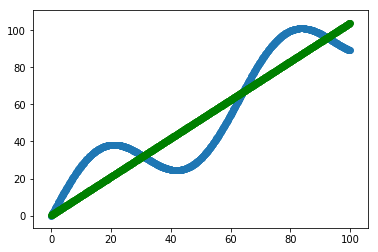
\includegraphics[width=.9\linewidth]{images/trained_model.png}
\end{center}
\end{center}

\section*{MNIST and TensorFlow}
\label{sec:orgabd66b0}
\subsection*{Introduction}
\label{sec:orgaae77bc}
\begin{itemize}
\item MNIST is the hello world of machine learning
\item Simple computer vision dataset, consists of images of handwritten digits
\item We are going to train a model to predict what the digits are
\end{itemize}

\begin{center}
\begin{center}

\includegraphics[width=.9\linewidth]{images/MNIST.png}
\end{center}
\end{center}
\subsubsection*{Importing MNIST Data}
\label{sec:org8741e9f}

To download and read in the data automatically:

\begin{minted}[]{python}
from tensorflow.examples.tutorials.mnist import input_data
mnist = input_data.read_data_sets("MNIST_data/", one_hot=True)
\end{minted}

One hot encoding
\begin{itemize}
\item labels have been converted to a vector of length equal to number of classes.
\item the ith element is 1, rest are 0. E.g. Digit 1: \([0,1,\dots]\)
\end{itemize}
\subsubsection*{MNIST Data}
\label{sec:org247944f}
The MNIST data is split into three parts:
\begin{enumerate}
\item 55,000 data points of training data (\texttt{mnist.train})
\item 10,000 data points of test data (\texttt{mnist.test})
\item 5,000 data points of validation data (\texttt{mnist.validation})
\end{enumerate}

Every MNIST data has 2 parts:
\begin{enumerate}
\item an image of a handwritten digit (call it "x")
\item corresponding label (call it "y")
\end{enumerate}
\subsection*{Softmax Regression}
\label{sec:org0ad7ebb}
\subsubsection*{Overview}
\label{sec:orgcacafd9}
\begin{center}
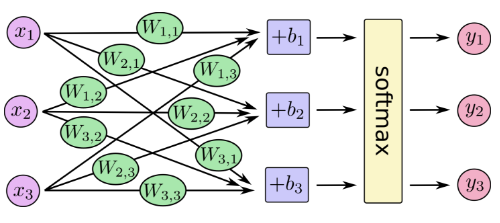
\includegraphics[width=.9\linewidth]{images/softmax_1.png}
\end{center}
\subsubsection*{Overview (1)}
\label{sec:org1f731ae}
\begin{center}
\begin{center}
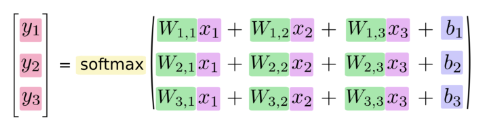
\includegraphics[width=.9\linewidth]{images/softmax_2.png}
\end{center}
\end{center}

\begin{center}
\begin{center}
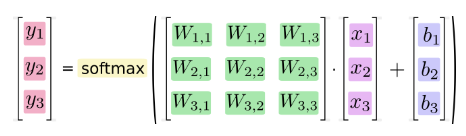
\includegraphics[width=.9\linewidth]{images/softmax_3.png}
\end{center}
\end{center}
\subsubsection*{Defining Our Model}
\label{sec:orge57a8ea}
\begin{itemize}
\item multiply 784-dimensional vectors by \(W\) to produce 10-dimensional vectors of evidence
\end{itemize}
\begin{minted}[]{python}
x = tf.placeholder(tf.float32, [None, 784])
W = tf.Variable(tf.zeros([784, 10]))
b = tf.Variable(tf.zeros([10]))

y = tf.nn.softmax(tf.matmul(x, W) + b)
\end{minted}
\begin{itemize}
\item multiply \texttt{x} with \texttt{W} in that order as \texttt{x} has shape \texttt{[None, 784]} and \texttt{W} has shape \texttt{[784, 10]}
\item Small trick to deal with \texttt{x} being a 2D tensor with multiple inputs.
\end{itemize}
\subsubsection*{Training}
\label{sec:org2b67b4a}
Use \textbf{cross-entropy} to determine loss of model:
$$H_{y'}=-\sum_{i} y_i' \log(y_i)$$

Where:
\begin{itemize}
\item \(y\) is our predicted probability distribution
\item \(y'\) is the true distribution (one-hot vector with digit labels)
\end{itemize}
\subsubsection*{Training (1)}
\label{sec:org9c93a62}
Need a placeholder to implement cross entropy:

\begin{minted}[]{python}
y_ = tf.placeholder(tf.float32, [None, 10])
cross_entropy = tf.reduce_mean(-tf.reduce_sum(y_ * tf.log(y), 
                                              reduction_indices = [1]))
\end{minted}

\texttt{tf.reduce\_sum} computes the sum of elements across dimensions of a tensor

\begin{minted}[]{python}
# 'x' is [[1, 1, 1]
#         [1, 1, 1]]
tf.reduce_sum(x) ==> 6
tf.reduce_sum(x, 0) ==> [2, 2, 2]
tf.reduce_sum(x, 1) ==> [3, 3]
\end{minted}
\subsubsection*{Training (2)}
\label{sec:org72e8f71}

\begin{minted}[]{python}
train_step = tf.train.GradientDescentOptimizer(0.5).minimize(cross_entropy)

sess = tf.Session()
sess.run(tf.global_variables_initializer())
for _ in range(400):
    batch_xs, batch_ys = mnist.train.next_batch(100)
    sess.run(train_step, feed_dict={x: batch_xs, y_: batch_ys})
\end{minted}

Using small batches of random data is called \textbf{stochastic training}, it is more
feasible than training on the entire data set
\subsubsection*{Evaluating Our Model}
\label{sec:orgb7d34b0}

\begin{itemize}
\item \texttt{tf.argmax} is an extrememly helpful function that returns the index of the highest entry in a tensor along some axis.
\item \texttt{tf.argmax(y,1)} is predicted label while \texttt{tf.argmax(y\_, 1)} is the actual label
\item \texttt{tf.equal} to check if prediction matches the true
\end{itemize}

\begin{minted}[]{python}
correct_prediction = tf.equal(tf.argmax(y,1), tf.argmax(y_,1))
accuracy = tf.reduce_mean(tf.cast(correct_prediction, tf.float32))
print(sess.run(accuracy, feed_dict={x: mnist.test.images, y_: mnist.test.labels}))
\end{minted}

Approx 91\% is very bad, 6 digit ZIP code would have an accuracy rate of 57\% 
\subsection*{Convolutional Neural Network}
\label{sec:orgc5c9ed1}
\subsubsection*{Flowchart}
\label{sec:orgefb7b41}
\begin{center}
\begin{center}
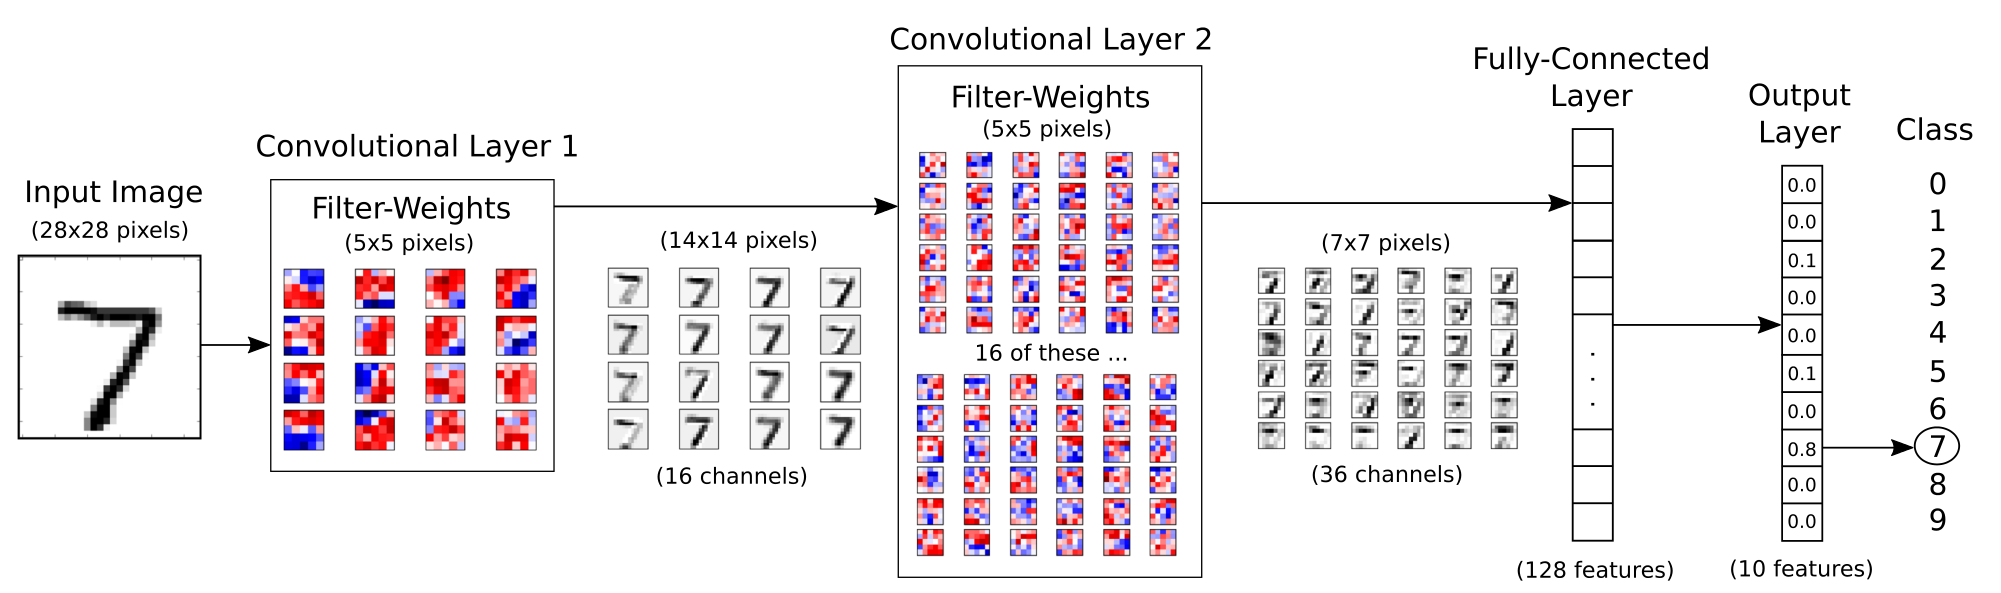
\includegraphics[width=.9\linewidth]{images/cnn_network_flowchart.png}
\end{center}
\end{center}
\subsubsection*{Introduction}
\label{sec:orge47eded}
\begin{itemize}
\item Convolutional Networks work by moving smaller filter across the input image
\item Filters are re-used for recognizing patters throughout the entire input image
\item This makes Convolutional Networks much more powerful than Fully-Connected
networks with the same number of variables
\end{itemize}
\subsubsection*{Features}
\label{sec:org1e45cce}
\begin{center}
\begin{center}
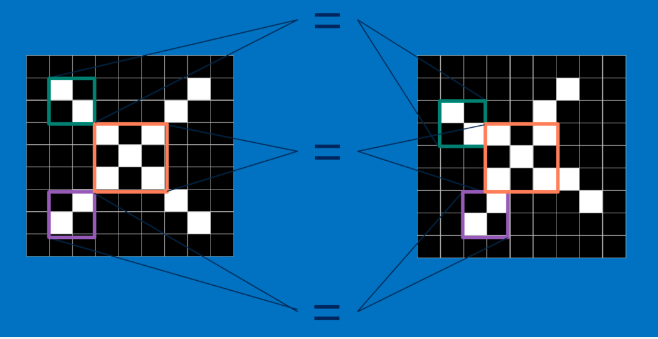
\includegraphics[width=.9\linewidth]{images/features.png}
\end{center}
\end{center}
\subsubsection*{Features (1)}
\label{sec:org733af8f}
\begin{center}
\begin{center}
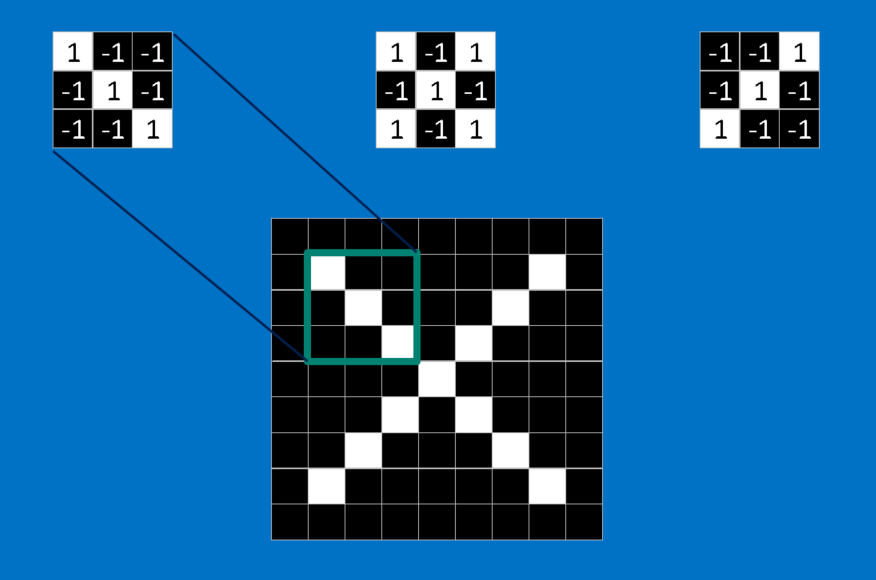
\includegraphics[width=.9\linewidth]{images/features_2.png}
\end{center}
\end{center}
\subsubsection*{Convolution}
\label{sec:orga45e5dd}
\begin{center}
\begin{center}
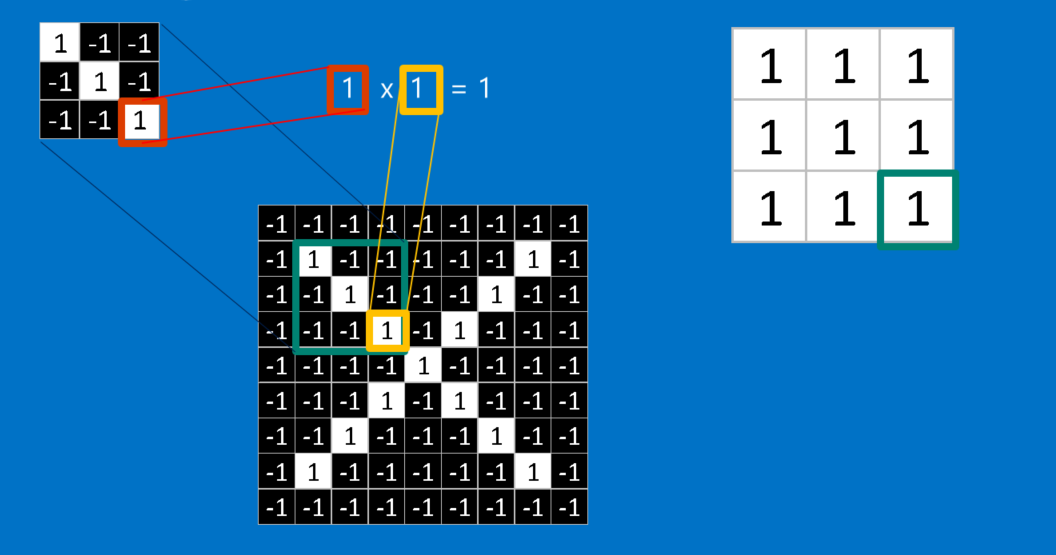
\includegraphics[width=.9\linewidth]{images/convolution.png}
\end{center}
\end{center}
\subsubsection*{Convolution (1)}
\label{sec:orgdb5e41d}
\begin{center}
\begin{center}
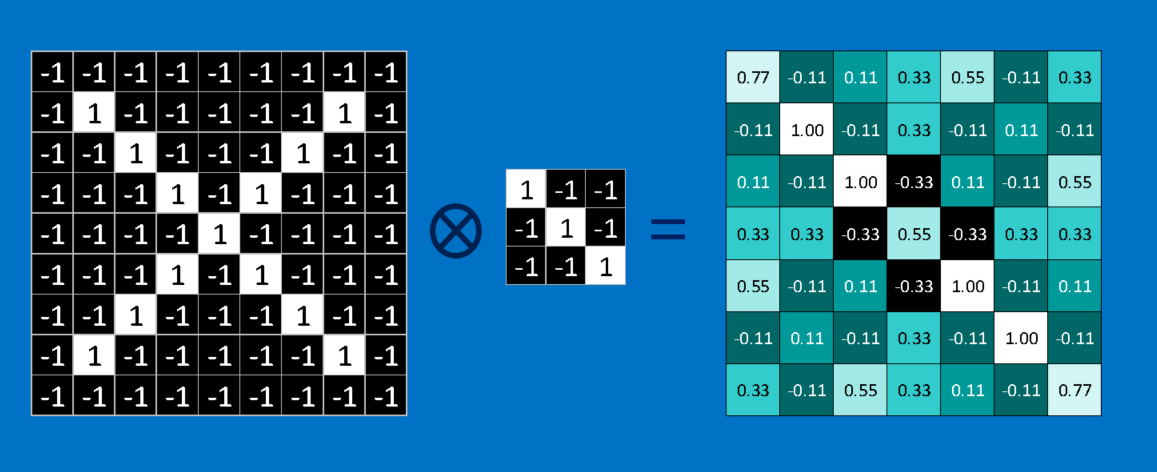
\includegraphics[width=.9\linewidth]{images/convolution_2.png}
\end{center}
\end{center}
\subsubsection*{Convolution (2)}
\label{sec:org06b67b1}
\begin{center}
\begin{center}
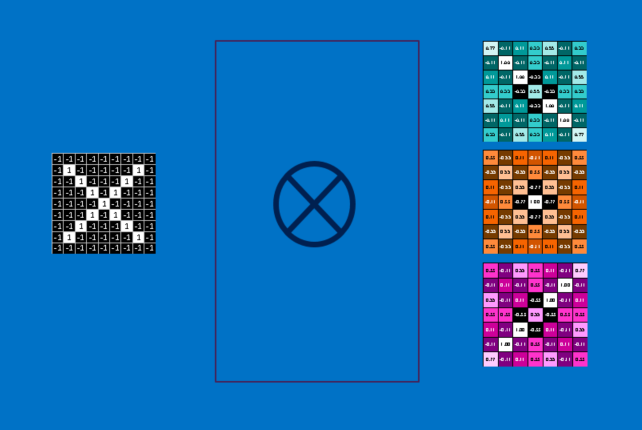
\includegraphics[width=.9\linewidth]{images/convolution_3.png}
\end{center}
\end{center}
\subsubsection*{Pooling}
\label{sec:org62a2a9f}
\begin{center}
\begin{center}
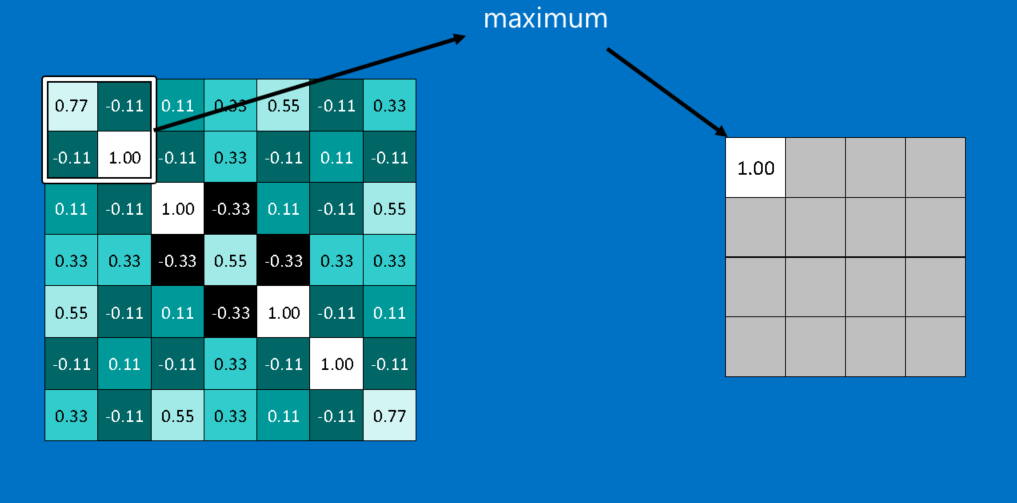
\includegraphics[width=.9\linewidth]{images/pooling.png}
\end{center}
\end{center}
\subsubsection*{Pooling (1)}
\label{sec:org897c601}
\begin{center}
\begin{center}
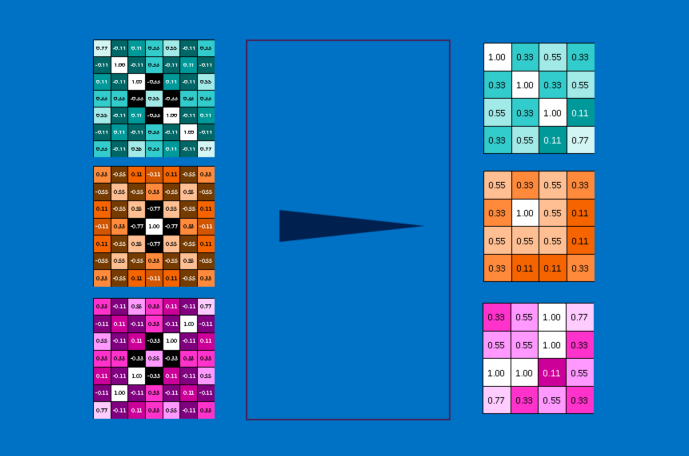
\includegraphics[width=.9\linewidth]{images/pooling_2.png}
\end{center}
\end{center}
\subsubsection*{Fully Connected Layers}
\label{sec:org528f0f2}
\begin{center}
\begin{center}
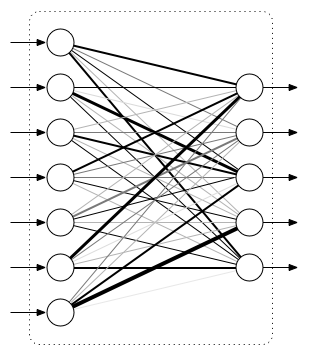
\includegraphics[width=.9\linewidth]{images/layers.png}
\end{center}
\end{center}
\subsubsection*{Hyper Parameters}
\label{sec:orga1d769f}
\begin{itemize}
\item Convolution:
\begin{itemize}
\item Number of features
\item Size of features
\end{itemize}
\item Pooling
\begin{itemize}
\item Window size
\item Window stride
\end{itemize}
\item Fully Connected
\begin{itemize}
\item number of neurons
\end{itemize}
\end{itemize}
\subsubsection*{Weight Initialization}
\label{sec:org3a7cbf2}
Helper functions to create ReLU neurons

\begin{minted}[]{python}
def weight_variable(shape):
  initial = tf.truncated_normal(shape, stddev=0.05)
  return tf.Variable(initial)

def new_biases(length):
    return tf.Variable(tf.constant(0.05, shape=[length]))
\end{minted}
\subsubsection*{Creating a new Convolutional Layer}
\label{sec:org923efce}

Input is a 4-dim tensor:
\begin{enumerate}
\item image number
\item y-axis of each image
\item x-axis of each image
\item channels of each image
\end{enumerate}

Output is another 4-dim tensor:
\begin{enumerate}
\item image number, same as input
\item y-axis of each image, might be smaller if pooling is used
\item x-axis of each image, might be smaller if pooling is used
\item channels produced by the convolutional filters
\end{enumerate}
\subsubsection*{Helper Function for Creating a New Layer}
\label{sec:orgacaf864}

\begin{minted}[]{python}

def new_conv_layer(input,              # The previous layer.
                   num_input_channels, # Num. channels in prev. layer.
                   filter_size,        # Width and height of each filter.
                   num_filters,        # Number of filters.
                   use_pooling=True):  # Use 2x2 max-pooling.
    # ...

    return layer, weights
\end{minted}
\subsubsection*{Flattening a Layer}
\label{sec:org64df0cd}

\begin{itemize}
\item convolutional layer produces an output tensor with 4 dimensions
\item fully connected layer will reduce 4-dim tensor to a 2-dim tensor that can be used as input to the fully connected layer
\end{itemize}

\begin{minted}[]{python}
def flatten_layer(layer):
    # ...

    # return both the flatten layer and number of features
    return layer_flat, num_features

\end{minted}
\subsubsection*{Creating a Fully-Connected Layer}
\label{sec:orgb210325}

Assumed that input is a 2-dim tensor of shape \texttt{[num\_images, num\_inputs]}, output is a 2-dim tensor of shape \texttt{[num\_images, num\_outputs]}

\begin{minted}[]{python}
def new_fc_layer(input,          # The previous layer.
                 num_inputs,     # Num. inputs from prev. layer.
                 num_outputs,    # Num. outputs.
                 use_relu=True): # Use Rectified Linear Unit (ReLU)?
    # create new weights and biases
    # calculate new layer
    # use ReLU?

    return layer
\end{minted}
\subsubsection*{Placeholder Variables}
\label{sec:org418fce8}

\begin{itemize}
\item \texttt{x} is the placeholder variable for input images
\begin{itemize}
\item data-type is set to \texttt{float32}
\item shape is set to \texttt{[None, img\_size\_flat]}
\end{itemize}
\item convolutional layers expect \texttt{x} to be encoded as a 4-dim tensor, so its shape
is \texttt{[num\_images, img\_height, img\_width, num\_channels]}
\item also have placeholder for true labels
\end{itemize}

\begin{minted}[]{python}
x = tf.placeholder(tf.float32, shape=[None, img_size_flat], name='x')
x_image = tf.reshape(x, [-1, img_size, img_size, num_channels])
y_true = tf.placeholder(tf.float32, shape=[None, num_classes], name='y_true')
y_true_cls = tf.argmax(y_true, axis=1)
\end{minted}

\subsubsection*{First Convolutional Layer}
\label{sec:org9f332af}

\begin{itemize}
\item takes \texttt{x\_image} as input and creates \texttt{num\_filters1} different filters
\begin{itemize}
\item each filter has width and height equal to filter\(_{\text{size1}}\)=
\end{itemize}
\item down sample the image so its half the size by using max-pooling
\end{itemize}
\begin{minted}[]{python}
layer_conv1, weights_conv1 = \
    new_conv_layer(input=x_image,
                   num_input_channels=num_channels,
                   filter_size=filter_size1,
                   num_filters=num_filters1,
                   use_pooling=True)
\end{minted}
\subsubsection*{Second Convolutional Layer}
\label{sec:org3a5488e}
\begin{itemize}
\item takes as input the output from the first convolutional layer
\item number of iunput channels = number of filters in the first convolutional layer
\end{itemize}

\begin{minted}[]{python}
layer_conv2, weights_conv2 = \
    new_conv_layer(input=layer_conv1,
                   num_input_channels=num_filters1,
                   filter_size=filter_size2,
                   num_filters=num_filters2,
                   use_pooling=True)
\end{minted}
\subsubsection*{Flatten Layer}
\label{sec:org76d712a}

\begin{itemize}
\item use output of convolutional layer as input to a fully-connected network, which
requires for the tensors to be reshaped to a 2-dim tensors
\end{itemize}

\begin{minted}[]{python}
layer_flat, num_features = flatten_layer(layer_conv2)
\end{minted}

\subsubsection*{Fully-Connected Layer 1}
\label{sec:org9ecbe0f}

\begin{minted}[]{python}
layer_fc1 = new_fc_layer(input=layer_flat,
                         num_inputs=num_features,
                         num_outputs=fc_size,
                         use_relu=True)
\end{minted}
\subsubsection*{Fully-Connected Layer 2}
\label{sec:org36d94a2}

\begin{minted}[]{python}
layer_fc2 = new_fc_layer(input=layer_fc1,
                         num_inputs=fc_size,
                         num_outputs=num_classes,
                         use_relu=False)
\end{minted}
\subsubsection*{Cost Function and Optimization Method}
\label{sec:orgd74cba9}

\begin{minted}[]{python}
y_pred = tf.nn.softmax(layer_fc2)
y_pred_cls = tf.argmax(y_pred, axis=1)
cross_entropy = tf.nn.softmax_cross_entropy_with_logits(logits=layer_fc2,
                                                        labels=y_true)
cost = tf.reduce_mean(cross_entropy)
optimizer = tf.train.AdamOptimizer(learning_rate=1e-4).minimize(cost)
correct_prediction = tf.equal(y_pred_cls, y_true_cls)
accuracy = tf.reduce_mean(tf.cast(correct_prediction, tf.float32))
\end{minted}

\subsection*{Saving and Restoring your model}
\label{sec:org47b7e5f}
\subsubsection*{Exporting the Model}
\label{sec:orgeb0b80c}
\begin{itemize}
\item We can export the model for use in our own applications
\item use \texttt{tf.train.Saver} to save the graph and the trained weights
\end{itemize}
\begin{minted}[]{python}
model_path = "./tmp/model.ckpt"
save_path = saver.save(sess, model_path) # saver is not declared???
print("Model saved in file: %s" % save_path)
\end{minted}

\subsubsection*{Restoring the Session}
\label{sec:org6026f43}
\begin{minted}[]{python}
saver = tf.train.Saver()
model_path = "./tmp/model.ckpt"
with tf.Session() as sess:
  sess.run(tf.global_variables_initializer())
  saver.restore(sess, model_path)
  print("Accuracy:", accuracy.eval({x: mnist.test.images, y_: mnist.test.labels}))
\end{minted}
\subsection*{Toy Program}
\label{sec:org07f6f43}
\begin{center}
\begin{center}
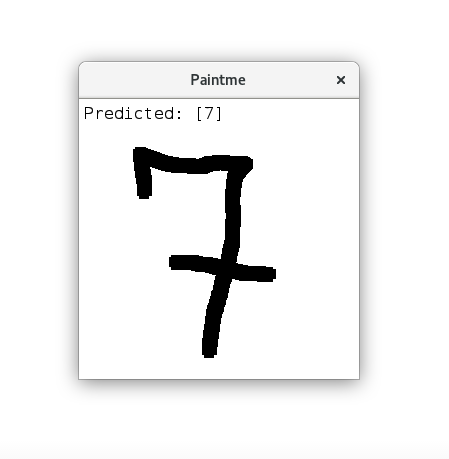
\includegraphics[width=.9\linewidth]{images/toy_program.png}
\end{center}
\end{center}
\section*{References}
\label{sec:org9b52b7f}
\begin{itemize}
\item \href{https://github.com/PythonWorkshop/intro-to-tensorflow/blob/master/MathPrimer/Math\%20primer\%20for\%20ML\%20\%26\%20TensorFlow\%20workshop.ipynb}{Machine Learning Primer}
\item \url{http://brohrer.github.io/how\_convolutional\_neural\_networks\_work.html}
\item \url{https://www.tensorflow.org/get\_started/mnist/beginners}
\item \url{https://www.tensorflow.org/get\_started/mnist/pros}
\item \url{https://github.com/Hvass-Labs/TensorFlow-Tutorials}
\end{itemize}

\section*{Thank You}
\label{sec:org5b7e8f2}
Emacs 25.2.1 (Org mode 9.0.9)
\end{document}
